% Paquets généraux
\documentclass[a4paper,12pt,titlepage]{article}
\usepackage[T1]{fontenc}
\usepackage[utf8]{inputenc}
\usepackage[french]{babel}
\usepackage[gen]{eurosym}
%\usepackage[dvips]{graphicx}
\usepackage{fancyhdr}
\usepackage{pdfpages} 
\usepackage{multido}
\usepackage{hyperref}
%\usepackage{textcomp}
%\usepackage{aeguill}
\usepackage{schemabloc}
\usepackage[bitstream-charter]{mathdesign}
\usepackage{minted}

\newcommand{\id}{71}
\newcommand{\nom}{Théorie des mécanismes}
\newcommand{\sequence}{04}
\newcommand{\nomsequence}{Liaisons entre les solides}
\newcommand{\num}{02}
\newcommand{\type}{KH}
\newcommand{\descrip}{Liaisons équivalentes, hyperstatisme, liaisons en série et en parallèle, théorie des graphes}
\newcommand{\competences}{B2-12: Proposer une modélisation des liaisons avec leurs caractéristiques géométriques. \\ &  B2-13: Proposer un modèle cinématique paramétré à partir d'un système réel, d'une maquette numérique ou d'u \\ &  B2-17: Simplifier un modèle de mécanisme. \\ &  B2-18: Modifier un modèle pour le rendre isostatique. \\ &  C1-04: Proposer une démarche permettant d'obtenir une loi entrée-sortie géométrique.  \\ &  C2-05: Caractériser le mouvement d'un repère par rapport à un autre repère. \\ &  C2-06: Déterminer les relations entre les grandeurs géométriques ou cinématiques. }
\newcommand{\nbcomp}{7}
\newcommand{\systemes}{}
\newcommand{\systemesnum}{}
\newcommand{\systemessansaccent}{}
\newcommand{\ilot}{2}
\newcommand{\ilotstr}{02}
\newcommand{\dossierilot}{\detokenize{Ilot_02 }}


\newcommand{\auteurun}{Renaud Costadoat}
\newcommand{\auteurdeux}{Françoise Puig}
\newcommand{\institute}{Lycée Dorian}


\usepackage{color}
\usepackage{xcolor}
\usepackage{colortbl}
\usepackage{helvet}
\usepackage[frenchmath]{newtxsf} % for sans serif symbols
\renewcommand{\familydefault}{\sfdefault}
%\usepackage{amsfonts}
%\usepackage{amsmath}
%\usepackage{lmodern}
\usepackage{mathastext}
%\usepackage{xspace}
\usepackage{varioref}
\usepackage{tabularx}
%\usepackage{floatflt}
\usepackage{graphics}
\usepackage{wrapfig}
\usepackage{textcomp}
\usepackage{tikz}
\usepackage{wrapfig}
\usepackage{gensymb}
\usepackage[european]{circuitikz}
\usetikzlibrary{babel}
\usepackage{ifthen}
\usepackage{cancel}
\usepackage{etoolbox}
\usepackage{multirow}
%\usepackage{boxedminipage}
\definecolor{gris25}{gray}{0.75}
\definecolor{bleu}{RGB}{18,33,98}
\definecolor{bleuf}{RGB}{42,94,171}
\definecolor{bleuc}{RGB}{231,239,247}
\definecolor{rougef}{RGB}{185,18,27}
\definecolor{rougec}{RGB}{255,188,204}%255,230,231
\definecolor{vertf}{RGB}{103,126,82}
\definecolor{vertc}{RGB}{220,255,191}
\definecolor{forestgreen}{rgb}{0.13,0.54,0.13}
\definecolor{blcr}{rgb}{0.59,0.69,0.84}
\definecolor{blfr}{rgb}{0.32,0.51,0.75}
\definecolor{orfr}{rgb}{0.90,0.42,0.15}
\definecolor{orcr}{rgb}{0.90,0.65,0.50}
\definecolor{orangef}{rgb}{0.659,0.269,0.072}
\definecolor{orange}{rgb}{0.58,0.35,0.063}
\definecolor{orangec}{rgb}{0.43,0.32,0.25}
\definecolor{rcorrect}{rgb}{0.6,0,0}
\definecolor{sequence}{rgb}{0.75,0.75,0.75}
\definecolor{competences}{rgb}{0.61,0.73,0.35}
\definecolor{grisf}{HTML}{222222}
\definecolor{grisc}{HTML}{636363}
\definecolor{normal}{HTML}{4087c4}
\definecolor{info}{HTML}{5bc0de}
\definecolor{success}{RGB}{92,184,92}
\definecolor{warning}{RGB}{240,173,78}
\definecolor{danger}{RGB}{217,83,79}
\hypersetup{                    % parametrage des hyperliens
    colorlinks=true,                % colorise les liens
    breaklinks=true,                % permet les retours à la ligne pour les liens trop longs
    urlcolor= blfr,                 % couleur des hyperliens
    linkcolor= orange,                % couleur des liens internes aux documents (index, figures, tableaux, equations,...)
    citecolor= forestgreen                % couleur des liens vers les references bibliographiques
    }

% Mise en page
\pagestyle{fancy}

\setlength{\hoffset}{-18pt}

\setlength{\oddsidemargin}{0pt} 	% Marge gauche sur pages impaires
\setlength{\evensidemargin}{0pt} 	% Marge gauche sur pages paires
\setlength{\marginparwidth}{00pt} 	% Largeur de note dans la marge
\setlength{\headwidth}{481pt} 	 	% Largeur de la zone de tête (17cm)
\setlength{\textwidth}{481pt} 	 	% Largeur de la zone de texte (17cm)
\setlength{\voffset}{-18pt} 		% Bon pour DOS
\setlength{\marginparsep}{7pt}	 	% Séparation de la marge
\setlength{\topmargin}{-30pt} 		% Pas de marge en haut
\setlength{\headheight}{35pt} 		% Haut de page
\setlength{\headsep}{20pt} 		% Entre le haut de page et le texte
\setlength{\footskip}{30pt} 		% Bas de page + séparation
\setlength{\textheight}{700pt} 		% Hauteur de l'icone zone de texte (25cm)
\setlength\fboxrule{1 pt}
\renewcommand{\baselinestretch}{1}
\setcounter{tocdepth}{1}
\newcommand{\cadre}[2]
{\fbox{
  \begin{minipage}{#1\linewidth}
   \begin{center}
    #2\\
   \end{center}
  \end{minipage}
 }
}

\newcounter{num_quest} \setcounter{num_quest}{0}
\newcounter{num_rep} \setcounter{num_rep}{0}
\newcounter{num_cor} \setcounter{num_cor}{0}

\newcommand{\question}[1]{\refstepcounter{num_quest}\par
~\ \\ \parbox[t][][t]{0.15\linewidth}{\textbf{Question \arabic{num_quest}}}\parbox[t][][t]{0.93\linewidth}{#1}\par
}


\newcommand{\reponse}[1]
{\refstepcounter{num_rep}
\noindent
\rule{\linewidth}{.5pt}
\textbf{Question \arabic{num_rep}:}
\multido{\i=1+1}{#1}{~\ \\}
}

\newcommand{\cor}
{\refstepcounter{num_cor}
\noindent
\rule{\linewidth}{.5pt}
\textbf{Question \arabic{num_cor}:} \\
}

\newcommand{\titre}[1]
{\begin{center}
\cadre{0.8}{\huge #1} 
\end{center}
}


% En tête et pied de page
\fancypagestyle{normal}{%
  \fancyhf{}
\lhead{\nom}
\rhead{
\includegraphics[width=2cm]{../../img/logo}\hspace{2pt}}
\ifdef{\auteurdeux}{\lfoot{\auteurun,\auteurdeux}}{\lfoot{\auteurun}}
\cfoot{Page \thepage}}

\fancypagestyle{correction}{%
  \fancyhf{}
  \lhead{\colorbox{danger}{\begin{minipage}{0.65\paperwidth} \textcolor{white}{\textbf{Correction}} \end{minipage}} }
  \rhead{
\includegraphics[width=2cm]{../../img/logo}}
  \ifdef{\auteurdeux}{\lfoot{\auteurun,\auteurdeux}}{\lfoot{\auteurun}}
  \rfoot{\colorbox{danger}{\begin{minipage}{0.5\paperwidth} \begin{flushright}\textcolor{white}{\textbf{Correction}}\end{flushright} \end{minipage}} }}

\renewcommand{\footrulewidth}{0.4pt}

\usepackage{eso-pic}
\newcommand{\BackgroundPic}{%
\put(0,0){%
\parbox[b][\paperheight]{\paperwidth}{%
\vfill
\begin{center}
\hspace{0.5cm}\vspace{0.5cm}

\includegraphics[width=\paperwidth,height=\paperheight,%
keepaspectratio]{../../img/fond3}%
\end{center}
\vfill
}}}

\newcommand{\BackgroundPicdeux}{%
\put(25,-30){%
\parbox[b][\paperheight]{\paperwidth}{%
\vfill
\begin{center}
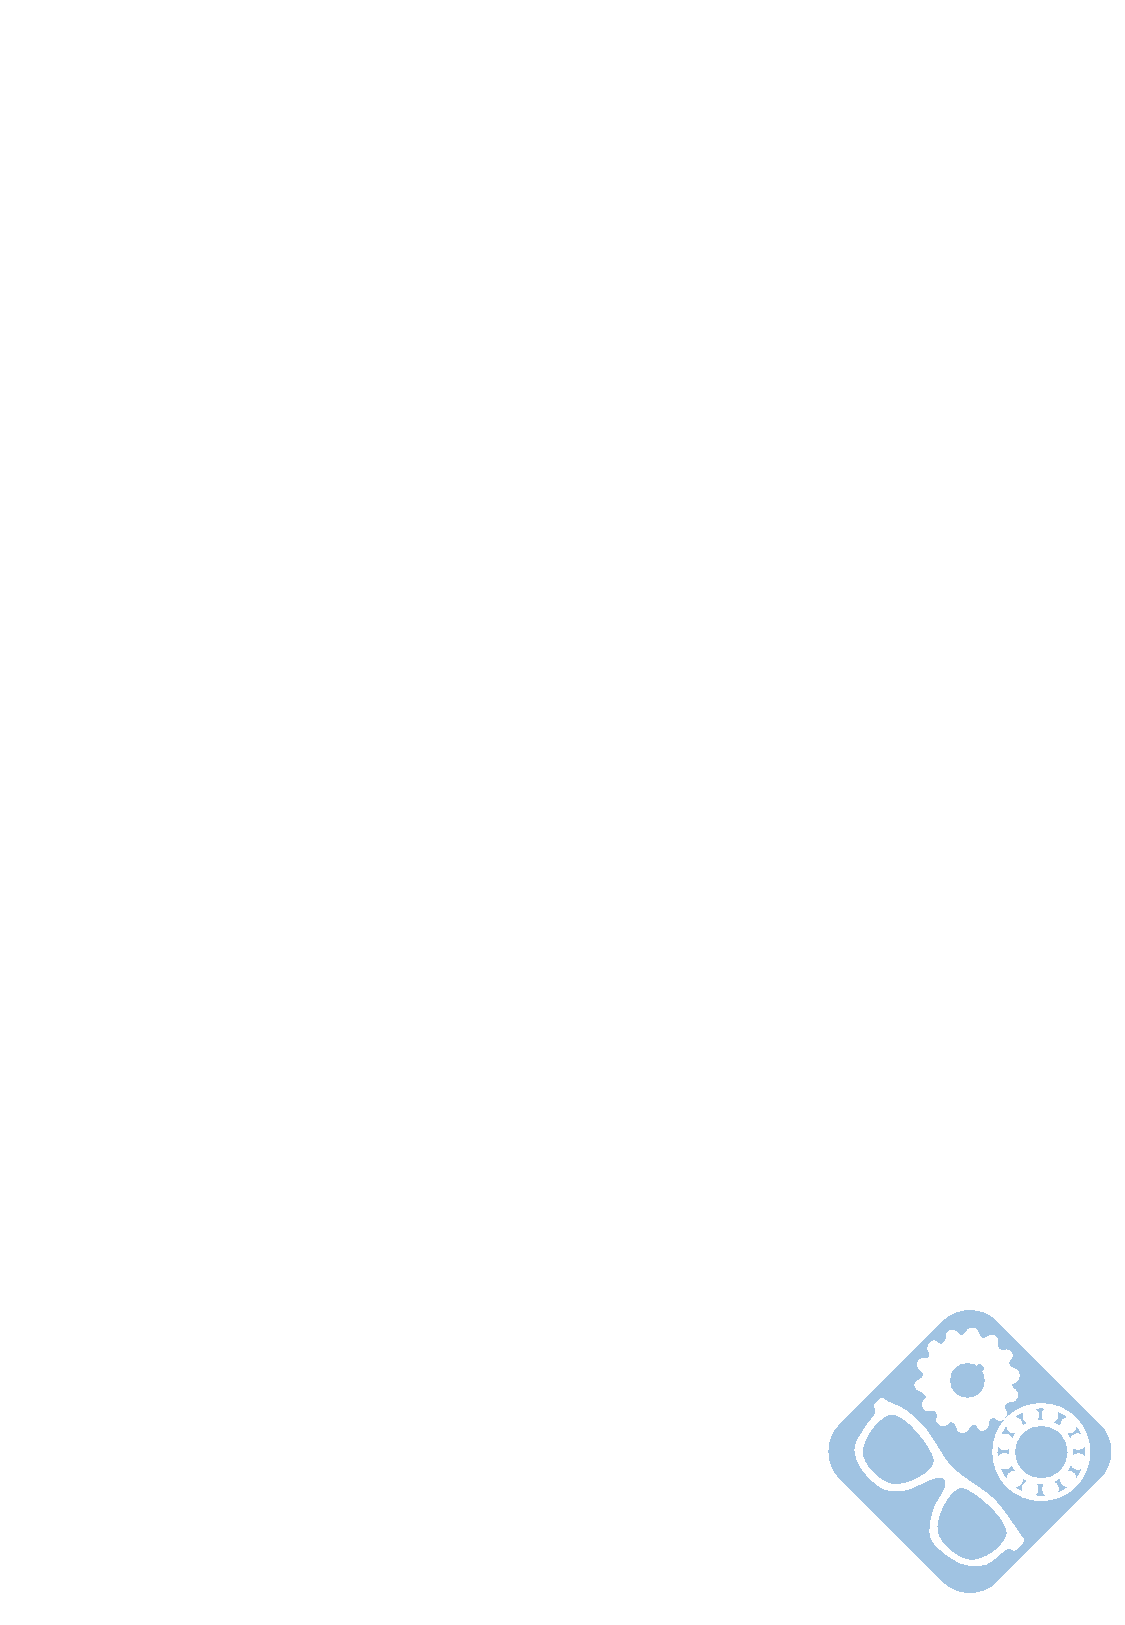
\includegraphics[width=\paperwidth,height=\paperheight,%
keepaspectratio]{../../img/fond4}%
\end{center}
\vfill
}}}

\begin{document}

\pagestyle{empty}

\vspace*{-3\baselineskip}

\AddToShipoutPicture*{\BackgroundPic}

\ifdef{\auteurdeux}{\begin{tabular}{>{\columncolor{gray!00}}m{.3\linewidth} m{.3\linewidth} >{\columncolor{gray!00}}m{.3\linewidth}}
Séquence : \sequence &  \multirow{3}{*}{\hspace{1cm}
\includegraphics[height=1.5cm]{../../img/logo}} &  \begin{flushright} \multirow{4}{*}{\hspace{1cm}\includegraphics[height=4cm]{img/qrcode}}\end{flushright}\\
Document : \type\num \\
 \institute \\
 \auteurun\\
 \auteurdeux
\end{tabular}}{\begin{tabular}{>{\columncolor{gray!00}}m{.3\linewidth} m{.3\linewidth} >{\columncolor{gray!00}}m{.3\linewidth}}
Séquence : \sequence &  \multirow{3}{*}{\hspace{1cm}
\includegraphics[height=1.5cm]{../../img/logo}} &  \begin{flushright} \multirow{4}{*}{\hspace{1cm}\includegraphics[height=4cm]{img/qrcode}}\end{flushright}\\
Document : \type\num \\
 \institute \\
 \auteurun
\end{tabular}}

\vspace{1cm}

\ifdef{\prive}{\begin{center}\colorbox{danger}{\Huge{Avec Correction}}\end{center}}{}

\begin{center}\huge{\nom}\end{center}

\vspace{2cm}

\ifdef{\imagedeux}{\begin{minipage}{0.49\linewidth}}{}
\begin{center}\includegraphics[height=5cm]{/home/renaud/Documents/Renaud/GitHub/django_education/systemes/\imageun}\end{center}
\ifdef{\imagedeux}{\end{minipage}\hfill
\begin{minipage}{0.49\linewidth}
\begin{center}\includegraphics[height=5cm]{/home/renaud/Documents/Renaud/GitHub/django_education/systemes/\imagedeux}\end{center}
\end{minipage}}{}

\vspace{5cm}


\begin{tabular}{p{.15\linewidth} >{\columncolor{white}}p{.8\linewidth}}
    \rowcolor{gray!20}
    Référence & S\sequence\ - \type\num \\
    Compétences & \competences \\
 	\rowcolor{gray!20}
    Description & \descrip \\
    Système & \systemes
  \end{tabular}

\newpage

\AddToShipoutPicture{\BackgroundPicdeux}

\pagestyle{normal}

\section{Tracer un trait}

Le but de ce travail va être de faire tracer un trait \og à main levée\fg\ à Simone afin de vérifier son aptitude à se passer d'une règle.

\begin{figure}[h!]
\begin{center}
  \resizebox{0.5\textwidth}{!}{\input{img/vue_bras.pdf_tex}}
  \caption{\label{fig01} Bras paramétré}
\end{center}
\end{figure}


\question{Tracer le graphe des liaisons de cette sous-partie de Simone.}

\question{Justifier qu'il s'agit d'un cycle ouvert et déterminer son degré d'hyperstatisme.}

On définit $x$ et $y$ tels que $\overrightarrow{AC}=x\cdot\vec{x}+y\cdot\vec{y}$.

On cherche à tracer la droite $y(x)=c\cdot x+d$ reliant les points $\left(\begin{array}{c}a+b\\0
\end{array}\right)_R$ et $\left(\begin{array}{c}0\\a+b
\end{array}\right)_R$.

\question{Déterminer $c$ et $d$ en fonction de $a$ et $b$.} 

\question{Déterminer $x$ et $y$ en fonction de $\alpha$, de $\beta$ et des dimensions du système.} 

\question{Déterminer $x$ et $y$ en fonction de $\theta$ et de $u=\left\|\overrightarrow{AC}\right\|$.} 

\question{Déterminer $u=\left\|\overrightarrow{AC}\right\|$ en fonction de $\theta$ et des dimensions du système.} 

\question{Déterminer $\alpha$ et $\beta$ en fonction de $\theta$, de $u=\left\|\overrightarrow{AC}\right\|$ et des dimensions du système. Et justifier que:
\begin{center}
$\alpha=\theta\pm\arccos\left(\dfrac{u^2+a^2-b^2}{2\cdot u\cdot a}\right)$ et $\beta=\theta-\alpha\pm\arccos\left(\dfrac{u^2+b^2-a^2}{2\cdot u\cdot b}\right)$
\end{center}
} 

\question{Tester le résultat à l'aide d'un code python.}

\section{Faire des squats}

Le but de ce travail va être de faire faire des \og squat\fg\ à Simone.

\begin{figure}[ht!]
\begin{minipage}{0.45\linewidth}
\begin{center}
 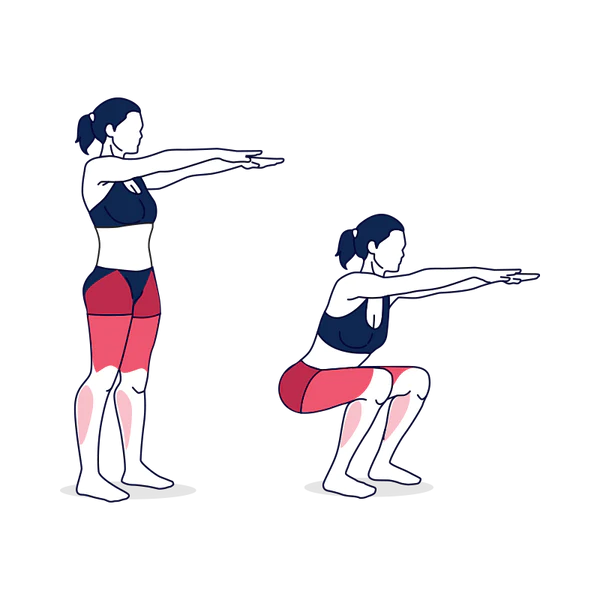
\includegraphics[width=0.8\linewidth]{img/squat}
\end{center}
\caption{\label{fig02} Mouvement de Squat}
\end{minipage}
\hfill
\begin{minipage}{0.45\linewidth}
\begin{center}
 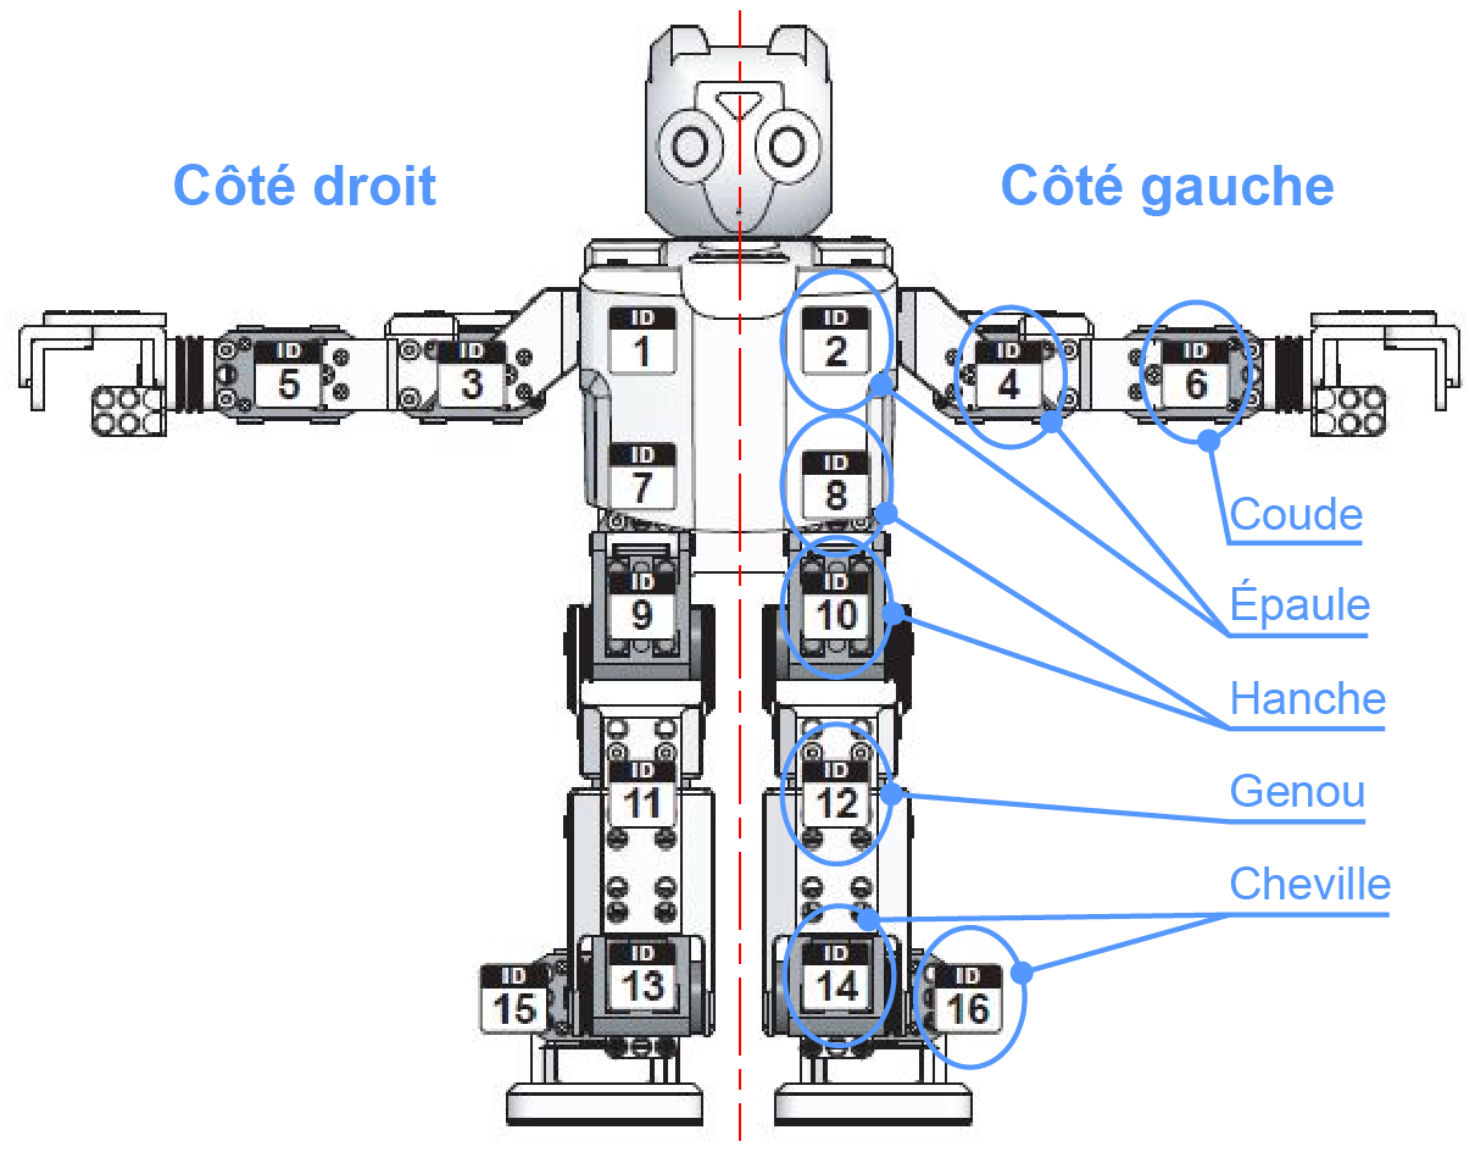
\includegraphics[width=0.9\linewidth]{img/structure_simone.png}
\end{center}
\caption{\label{fig03} Structure de Simone}
\end{minipage}
\end{figure}

\begin{figure}[h!]
\begin{center}
  \resizebox{0.4\textwidth}{!}{\input{img/squat_simone.pdf_tex}}
  \caption{\label{fig04} Bras paramétré}
\end{center}
\end{figure}

On notera respectivement $i_g$ et $i_d$ les pièces des jambes gauche et droite. On considérera que les deux pieds font partie de la classe équivalente \textit{sol}.

\question{Tracer le graphe des liaisons de cette sous-partie de Simone.}

\question{Justifier qu'il s'agit d'un cycle fermé et déterminer son degré d'hyperstatisme.}

\question{Proposer une modification d'une liaison pour rendre le système isostatique.}

\clearpage

\ifdef{\public}{\end{document}}{}

\newpage

\pagestyle{correction}\setcounter{section}{0}

\section{Correction}

\subsection{Tracer un trait}

\paragraph{Question 1:} ~\ \\

\begin{figure}[h!]
\begin{center}
  \resizebox{0.4\textwidth}{!}{\input{img/graphe_liaison_1.pdf_tex}}
  \caption{\label{fig05} Graphe de liaison 1}
\end{center}
\end{figure}

\paragraph{Question 2:} C'est un cycle ouvert car il n'y a pas de cycle fermé dans le graphe.

\paragraph{Question 3:}
 
$y(0)=d=a+b$, donc $d=a+b$.

$y(a+b)=c\cdot (a+b)+a+b=0$, donc $c=-1$

\paragraph{Question 4:}

$\overrightarrow{AC}=\overrightarrow{AB}+\overrightarrow{BC}$

$\overrightarrow{AC}=a\cdot\vec{x_1}+b\cdot\vec{x_2}$

$\overrightarrow{AC}=(a\cdot cos\alpha+b\cdot cos(\alpha+\beta))\vec{x_0}+(a\cdot sin\alpha+b\cdot sin(\alpha+\beta))\vec{y_0}$

Ainsi:
$\left\{\begin{array}{l}
x=a\cdot cos\alpha+b\cdot cos(\alpha+\beta)\\
y=a\cdot sin\alpha+b\cdot sin(\alpha+\beta)
\end{array}\right.$


\paragraph{Question 5:}

Ainsi:
$\left\{\begin{array}{l}
x=u\cdot cos\theta\\
y=u\cdot sin\theta
\end{array}\right.$

\paragraph{Question 6:} $u=\dfrac{a+b}{\sqrt{2}\cdot cos\left(\theta-\dfrac{\pi}{4}\right)}$

\begin{figure}[h!]
\begin{center}
  \resizebox{0.4\textwidth}{!}{\input{img/construction_u.pdf_tex}}
  \caption{\label{fig06} Construction pour u}
\end{center}
\end{figure}

\paragraph{Question 7:}

$\left\{\begin{array}{l}
u\cdot cos\theta=a\cdot cos\alpha+b\cdot cos(\alpha+\beta)\\
u\cdot sin\theta=a\cdot sin\alpha+b\cdot sin(\alpha+\beta)
\end{array}\right.$

$\left\{\begin{array}{l}
(b\cdot cos(\alpha+\beta))^2=(u\cdot cos\theta-a\cdot cos\alpha)^2\\
(b\cdot sin(\alpha+\beta))^2=(u\cdot sin\theta-a\cdot sin\alpha)^2
\end{array}\right.$

$b^2=(u\cdot cos\theta-a\cdot cos\alpha)^2+(u\cdot sin\theta-a\cdot sin\alpha)^2$

$b^2=(u\cdot cos\theta)^2+(a\cdot cos\alpha)^2-2\cdot u\cdot cos\theta\cdot a\cdot cos\alpha+(u\cdot sin\theta)^2+(a\cdot sin\alpha)^2-2\cdot u\cdot sin\theta\cdot a\cdot sin\alpha$

$2\cdot u\cdot a\cdot \left(sin\theta\cdot sin\alpha+cos\theta\cdot cos\alpha\right)=u^2+a^2-b^2$

$2\cdot u\cdot a\cdot cos(\theta-\alpha)=u^2+a^2-b^2$

$cos(\theta-\alpha)=\dfrac{u^2+a^2-b^2}{2\cdot u\cdot a}$

$\theta-\alpha=\pm\arccos\left((\dfrac{u^2+a^2-b^2}{2\cdot u\cdot a}\right)$

$\alpha=\theta\pm\arccos\left((\dfrac{u^2+a^2-b^2}{2\cdot u\cdot a}\right)$

On montre de même que:

$\left\{\begin{array}{l}
(a\cdot cos\alpha)^2=(u\cdot cos\theta-b\cdot cos(\alpha+\beta))^2\\
(a\cdot sin\alpha)^2=(u\cdot sin\theta-b\cdot sin(\alpha+\beta))^2
\end{array}\right.$

$a^2=(u\cdot cos\theta-b\cdot cos(\alpha+\beta))^2+(u\cdot sin\theta-b\cdot sin(\alpha+\beta))^2$

$a^2=u^2+b^2-2\cdot u\cdot cos\theta\cdot b\cdot cos(\alpha+\beta)-2\cdot u\cdot sin\theta\cdot b\cdot sin(\alpha+\beta)$

$a^2=u^2+b^2-2\cdot u\cdot b\cdot cos(\theta-(\alpha+\beta))$

$cos(\theta-(\alpha+\beta))=\dfrac{u^2+b^2-a^2}{2\cdot u\cdot b}$


$\beta=\theta-\alpha\pm\arccos\left(\dfrac{u^2+b^2-a^2}{2\cdot u\cdot b}\right)$

\paragraph{Question 8:}

\begin{minted}[xleftmargin=2em,linenos,firstnumber=1]{python}
import numpy as np
import matplotlib.pyplot as plt

a=45
b=65

theta=np.linspace(0,np.pi/2,100)
u=np.sqrt(2)/2*(a+b)/np.cos(theta-np.pi/4)
alpha=theta-np.arccos((u**2+a**2-b**2)/(2*u*a))
beta=theta-alpha+np.arccos((u**2-a**2+b**2)/(2*u*b))

x=a*np.cos(alpha)+b*np.cos(alpha+beta)
y=a*np.sin(alpha)+b*np.sin(alpha+beta)

plt.plot(x,y)
plt.show()
\end{minted}

\subsection{Faire des squats}

\paragraph{Question 1:} ~\ \\

\begin{figure}[h!]
\begin{center}
  \resizebox{0.7\textwidth}{!}{\input{img/graphe_liaison_2.pdf_tex}}
  \caption{\label{fig07} Graphe de liaison 2}
\end{center}
\end{figure}

\paragraph{Question 2:} 

\textit{Méthode statique:}

Il y a  6 liaisons pivot, donc $Ns=6\times 5=30$.

$rs=6\cdot (p-1)-m=6\times (6-1)-3=30-3=27$.

$h=3$

\textit{Méthode cinématique:}

Il y a  6 liaisons pivot, donc $Ic=6\times 1=6$.

Il n'y a qu'un cycle, donc $E=6$.

$h = m-Ic+E$

$h = 3-6+6=3$

\paragraph{Question 3:} On pourrait remplacer la liaison pivot d'axe $(A,\vec{z_0})$ par une linéaire annulaire d'axe $(A,\vec{z_0})$.

\end{document}
